\chapter{Applicazione}
\label{chapter:app}
Un altro aspetto chiave del progetto è l'applicazione Android, sviluppata per essere fonte per la 
raccolta di qualsiasi dato utile alla classificazione. Sintetizzando l'intero funzionamento è possibile 
raccogliere le funzionalità offerte nella
\begin{itemize}
    \item raccolta di dati per l'analisi dell'attività.
    \item raccolta di dati per l'apprendimento.
    \item raccolta di dati aggiuntivi.
\end{itemize}
\subsubsection{Compatibilità}
La compatibilità offerta è con tutte le versioni di Android che supportano la versione delle API 16 o superiore, nella pratica tutte
le versioni maggiori o uguali ad Android 4.1 rilasciato nel 2012. 
Nella pratica, al momento della stesura di questa relazione, ciò assicura il funzionamento dell'app sul 99,8\% dei dispositivi 
con questo sistema operativo.
\begin{figure}[H]
    \centering
    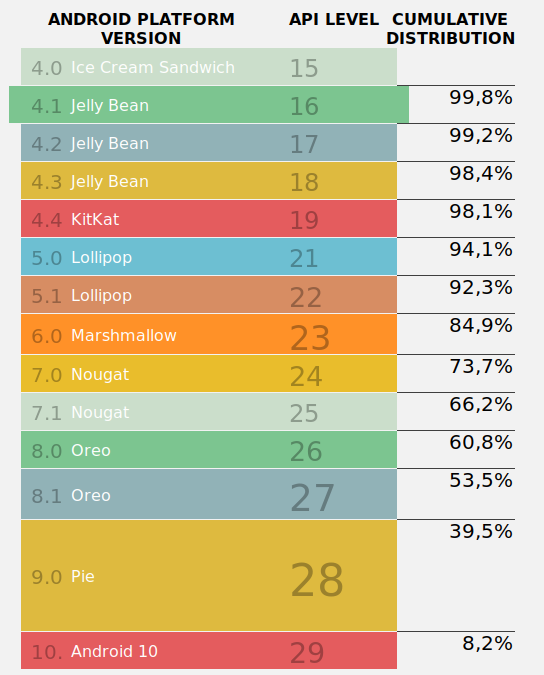
\includegraphics[scale = 0.40]{assets/images/android/compatibility.png}
    \caption{Distribuzione cumulativa delle versioni di Android}
    \label{fig:android-compatibility}
\end{figure}
\subsubsection{Linguaggi di sviluppo}
I linguaggi utilizzati sono stati \textit{Java} per quanto riguarda l'aspetto programmativo, mentre \textit{XML} per tutti i layout.
\subsubsection{Traduzioni}
L'intero applicativo, di cui segue la spiegazione, è stato interamente sviluppato con un supporto multilingua: italiano e inglese.

\section{Interfaccia}
Si è voluta dare un'interfaccia minimale sviluppata secondo le linee guida dell'ormai conosciuto Material Design.

\subsubsection{Material Design}
Con Material Design \cite{material} si intende un linguaggio visivo che \textit{sintetizza i principi classici 
del buon design utilizzando le nuove innovazioni della tecnologia e della scienza}.

L'intero linguaggio si basa sul concetto fisico "Materiale" di cui si vuole effettuare una trasposizione nel 
design di tutte le caratteristiche (luci, ombre, etc.) che lo definiscono nel mondo reale.

\subsubsection{Suddivisione per funzionalità}
Le 3 sezioni presenti suddividono con esattezza le 3 funzionalità offerte: 
l'analisi dell'attività, l'apprendimento di una attività e l'inserimento di informazioni aggiuntive.
\begin{figure}[H]
    \centering
    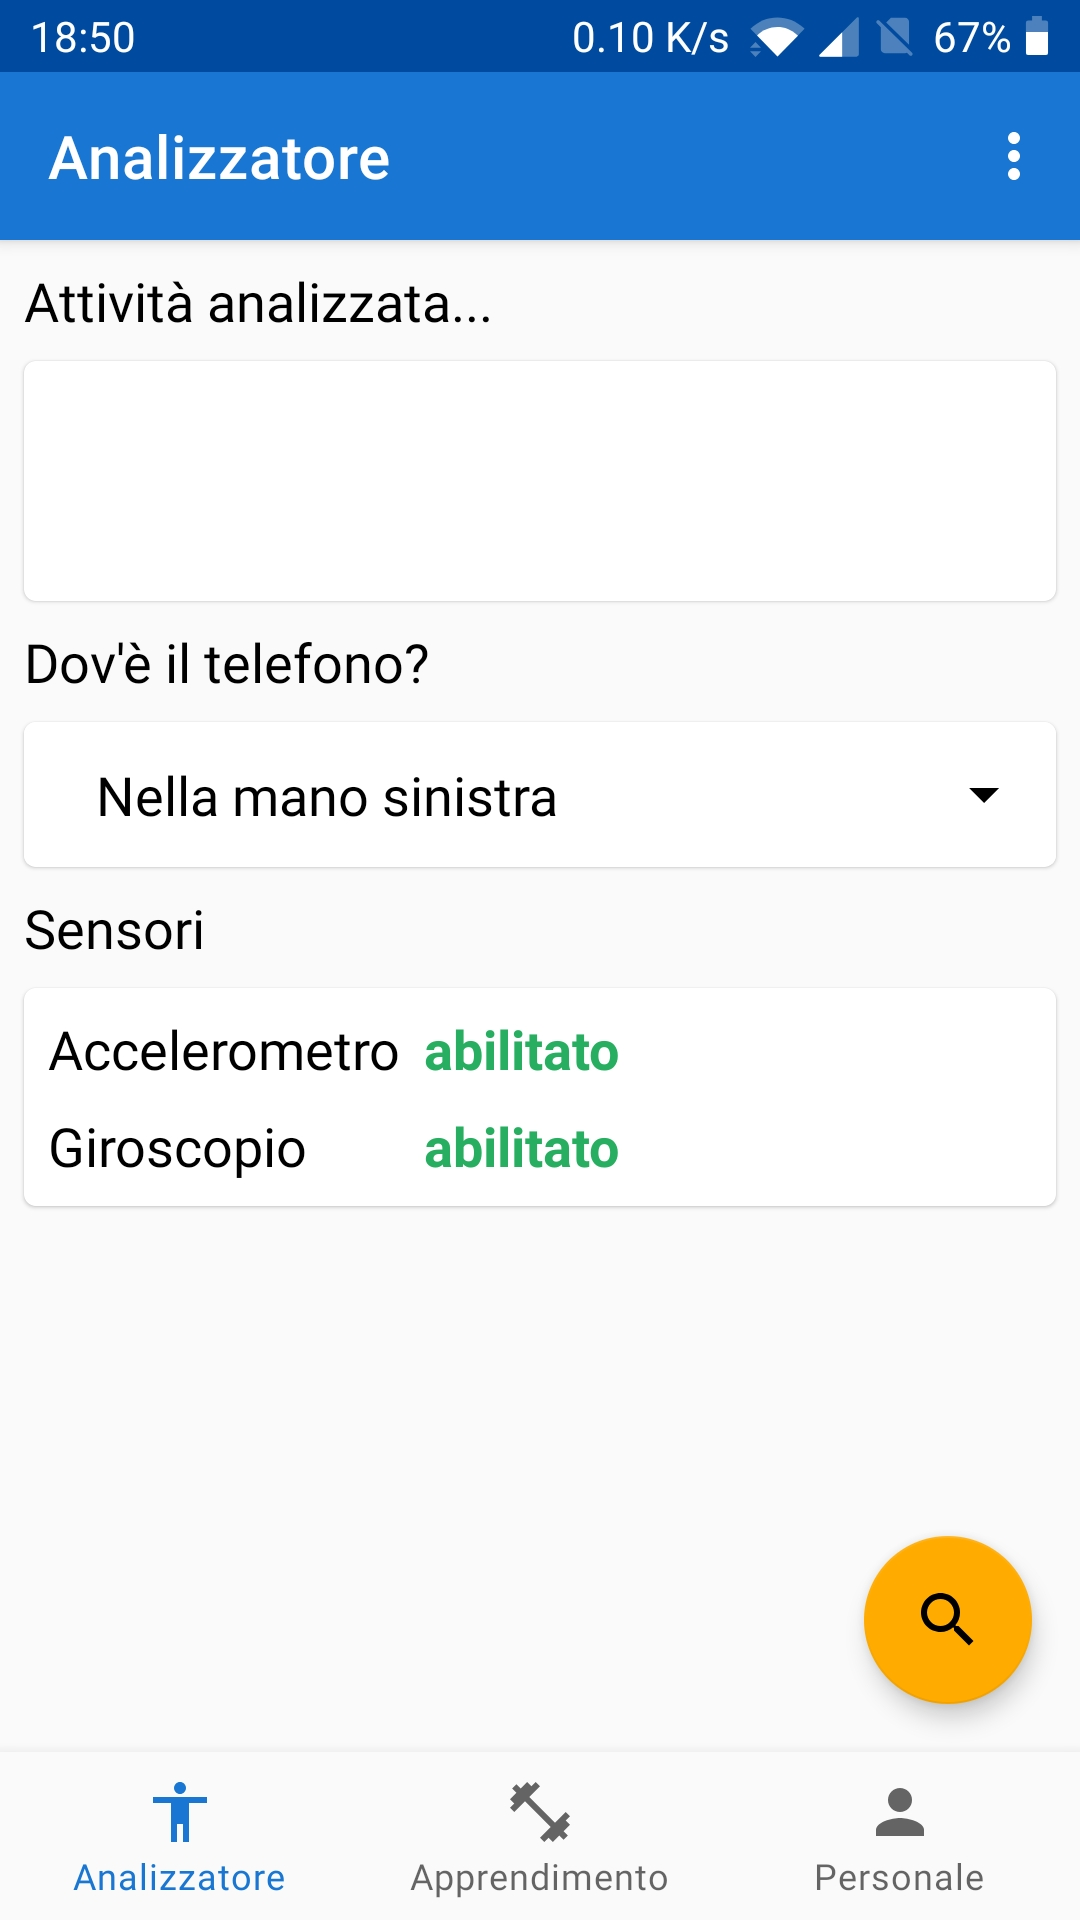
\includegraphics[scale = 0.1019]{assets/images/screenshots/1a_Init.jpg}
    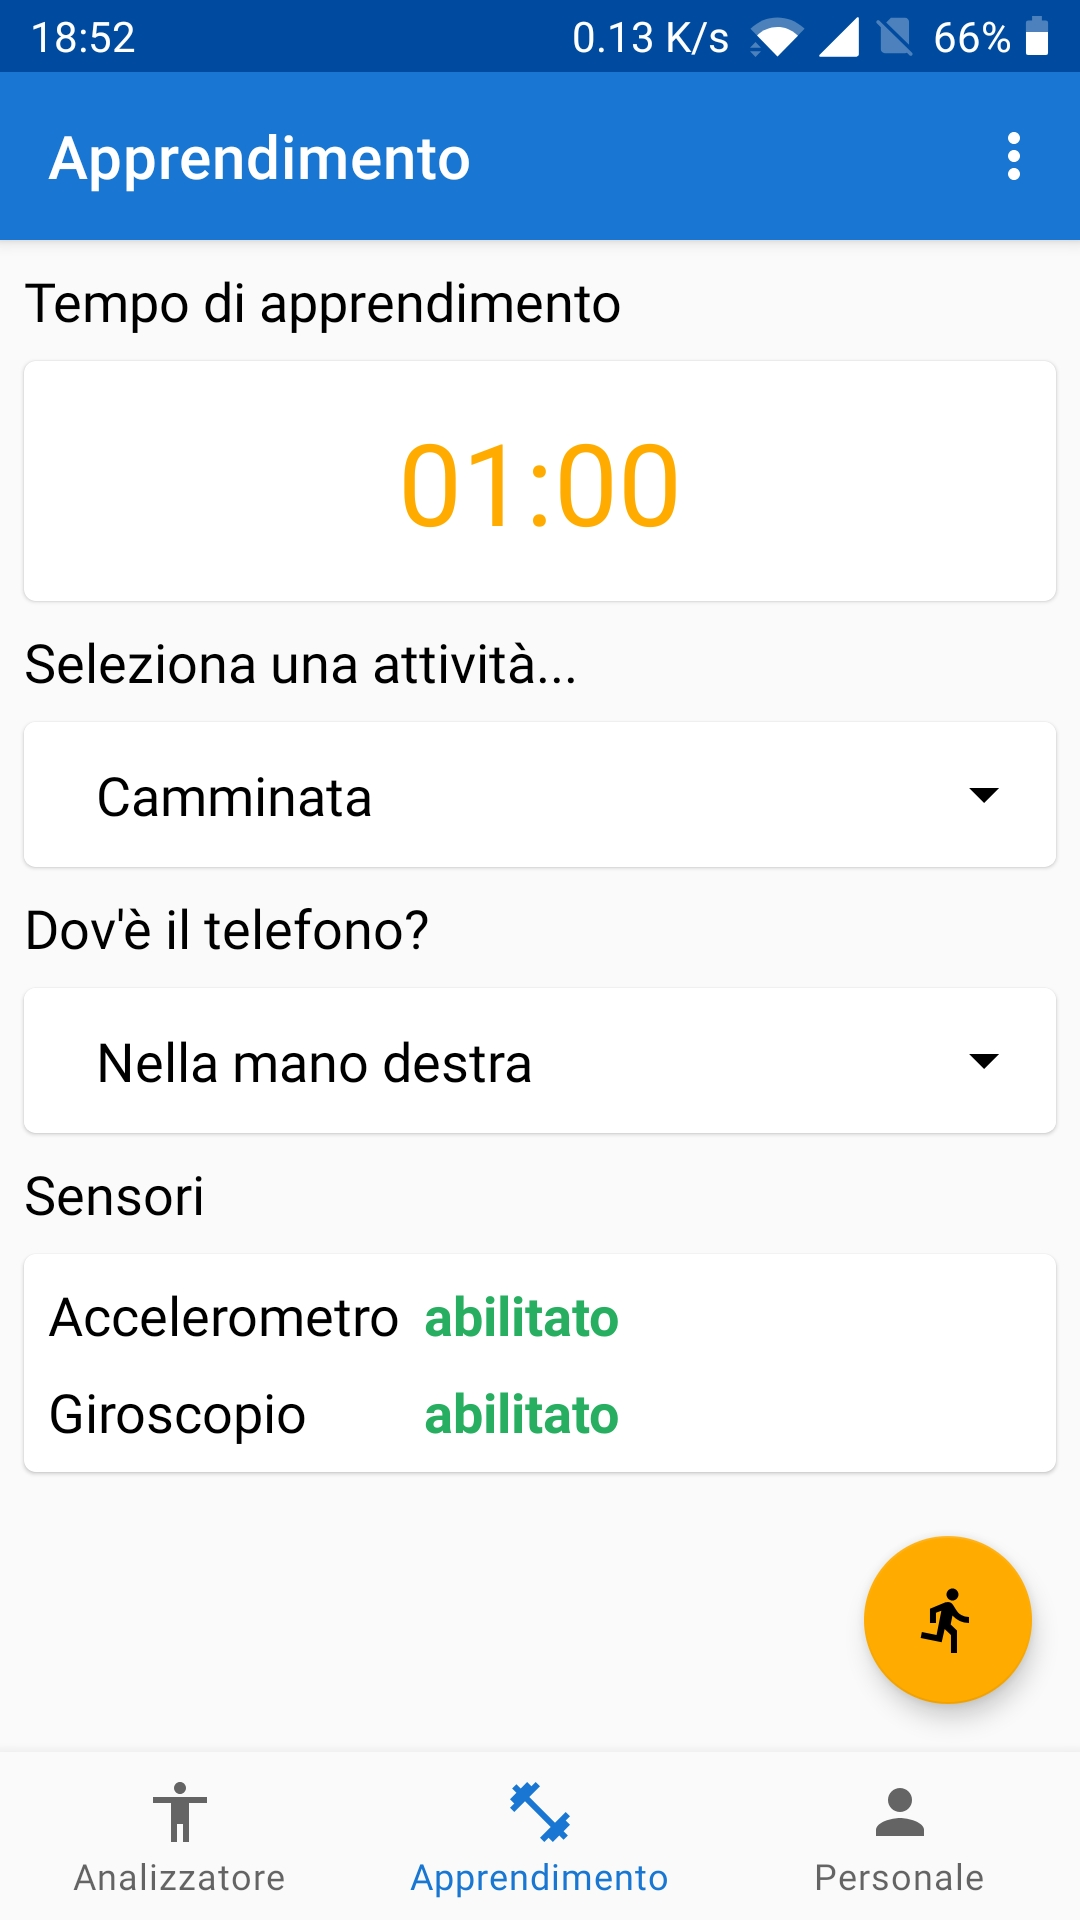
\includegraphics[scale = 0.1019]{assets/images/screenshots/2a_Init.jpg}
    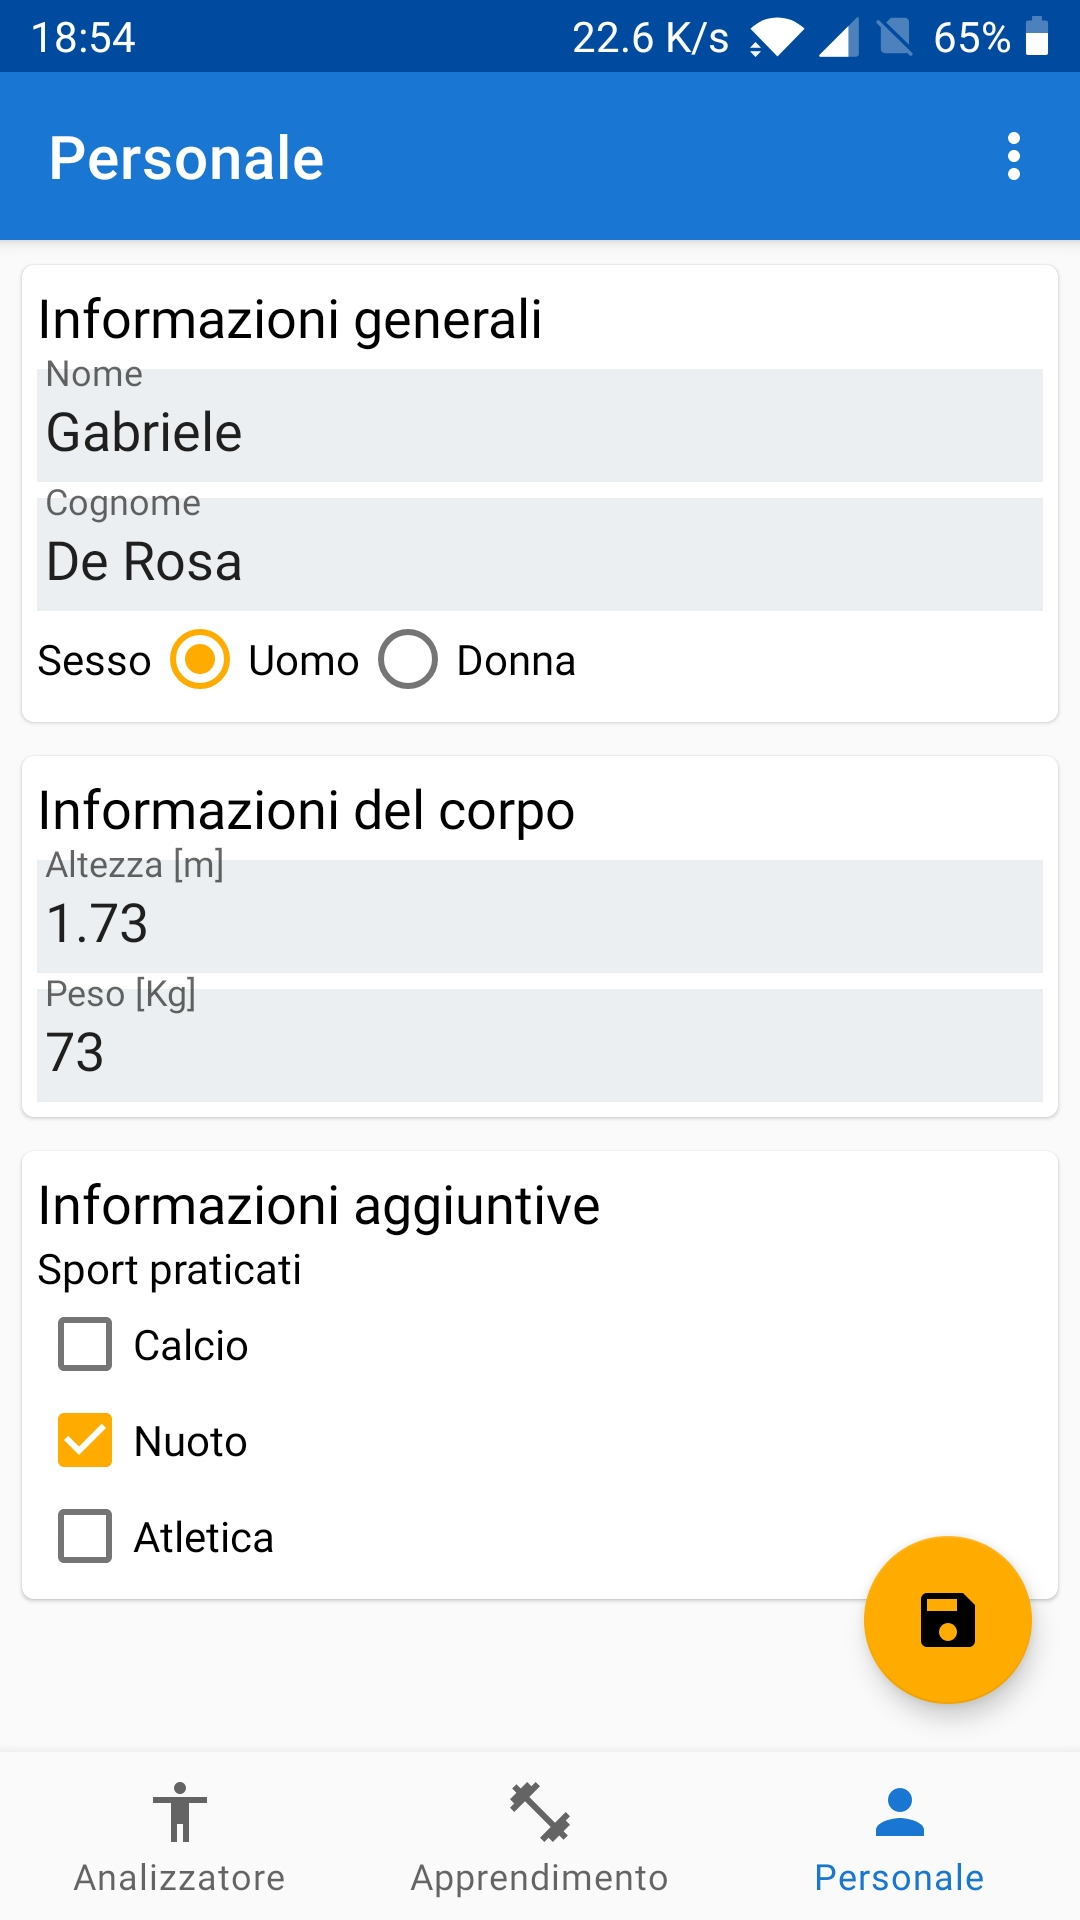
\includegraphics[scale = 0.1019]{assets/images/screenshots/3a_Init.jpg}
    \caption{Le 3 sezioni principali dell'applicazione}
    \label{fig:screenshots}
\end{figure}

\subsection{Sezione di analisi}
La sezione di analisi consente di testare l'efficacia del classificatore. Per meglio dire, è possibile avviare il processo di invio 
dei dati sensoriali al server ricevitore che, come abbiamo visto nella sezione \ref{section:receiver}, restituirà in risposta l'ipotesi.

L'insieme delle azioni svolte in questa sezione sono divisibili in 4 fasi.

\subsubsection{Fase 1: Inizializzazione}
In una prima fase l'applicazione scarica tramite l'utilizzo delle API (viste nella sezione \ref{section:api}) le informazioni relative
alle posizioni del dispositivo che sono disponibili e selezionabili.
L'utente ha quindi la possibilità di selezionare la posizione in cui desidera tenere il telefono durante l'esecuzione della attività ed 
in seguito avviare l'analisi.

\subsubsection{Fase 2: Preparazione}
All'avvio dell'analisi sarà inizializzato un servizio in foreground \cite{services} che si occuperà di svolgere tutte le azioni 
necessarie per le fasi seguenti. La UI continuerà ad essere aggiornata con le informazioni ricevute dal servizio.

Il primo obiettivo è quello di contattare il server per stabilire una connessione TCP ed iniziare lo scambio dati. 
Qualora la connessione avvenisse con successo passerà qualche altro secondo prima che i sensori inizino la raccolta dei dati.
Durante questo \textit{tempo di preparazione}, pensato appositamente in modo da consentire all'utente 
di prepararsi posizionando il dispositivo nella posizione selezionata, sarà mostrato un countdown.

\subsubsection{Fase 3: Analisi}
Allo scadere del countdown i sensori vengono abilitati. Ogni informazione raccolta è organizzata in un formato JSON organizzato in 
modo simile a quanto visto nell'esempio \ref{code:example-message-learning} ed inviata come messaggio.

\subsubsection{Fase 4: Predizione}
Durante il processo di analisi si ottengono numerose risposte dal server che manda sia messaggi di conferme che messaggi
contenenti le ipotesi sulla attività.
La predizione ottenuta è mostrata all'utilizzatore.

\begin{figure}[H]
    \centering
    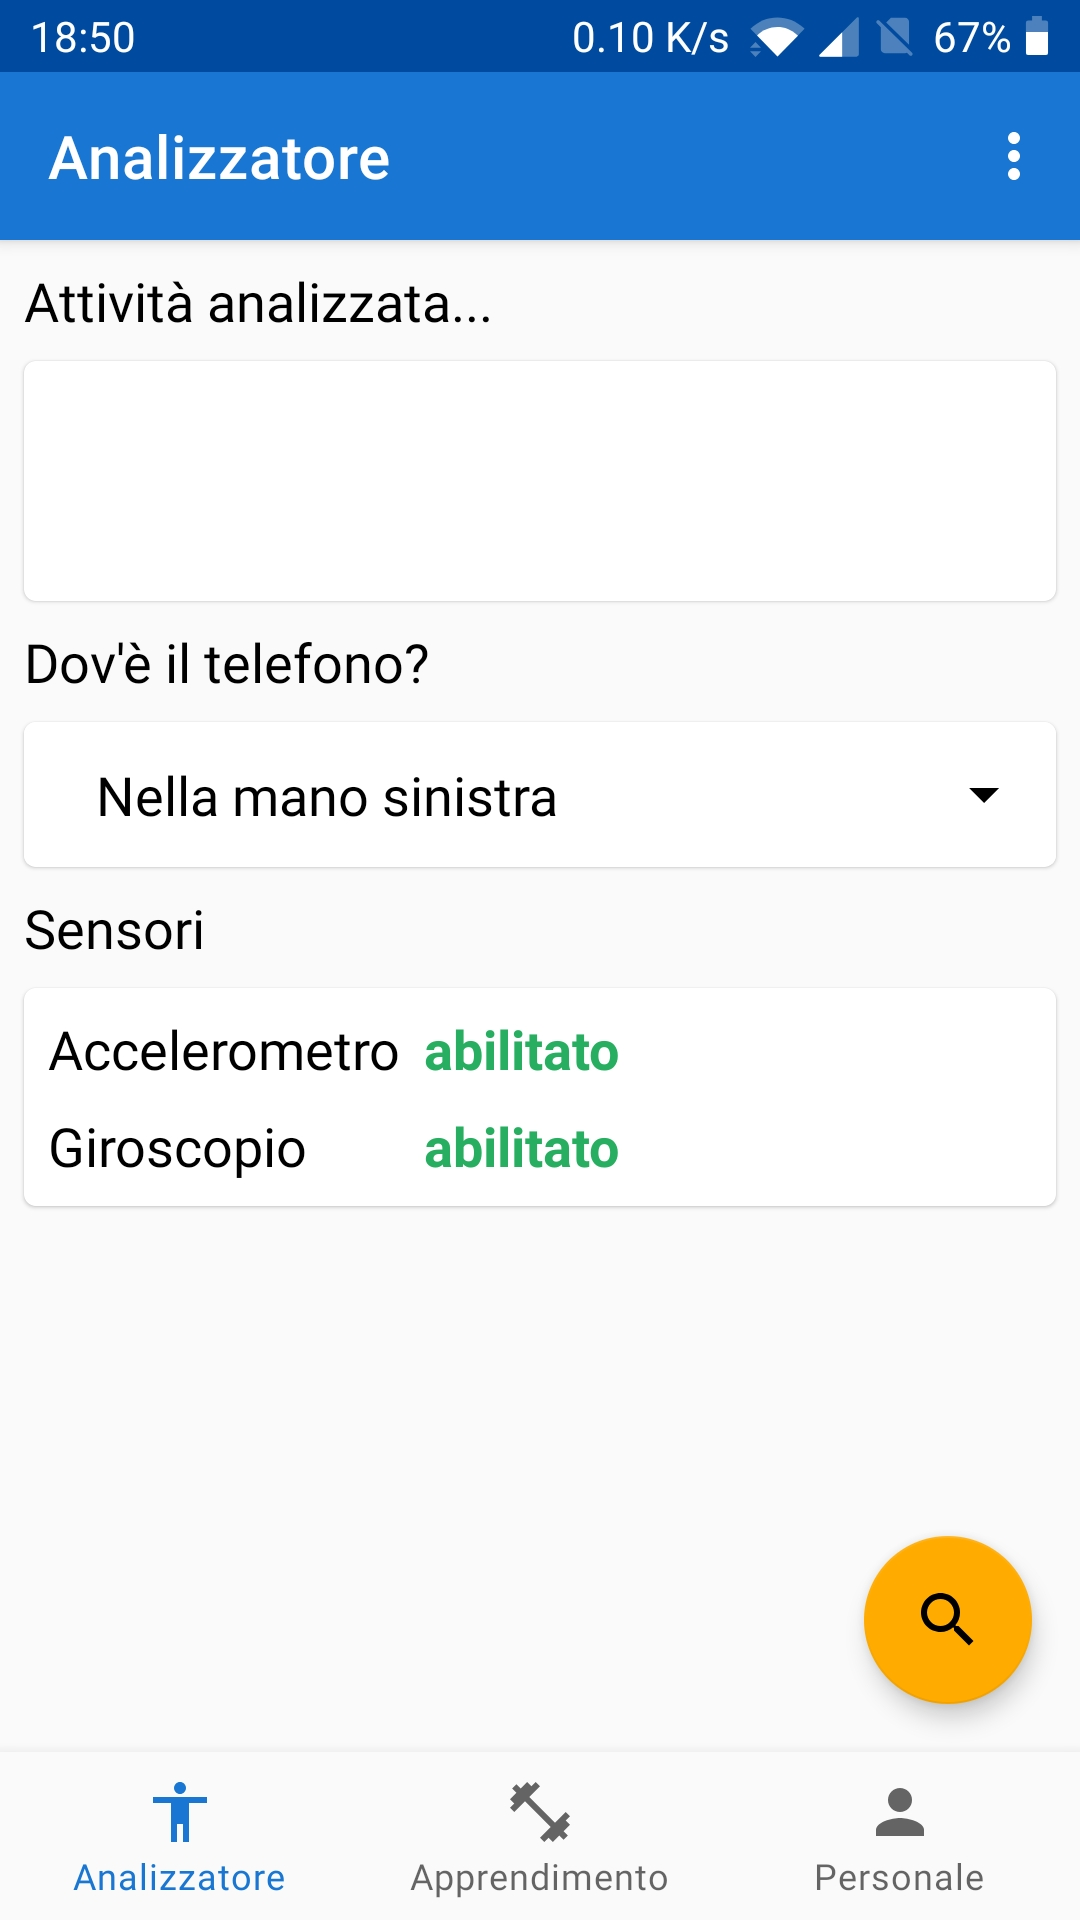
\includegraphics[scale = 0.1019]{assets/images/screenshots/1a_Init.jpg}
    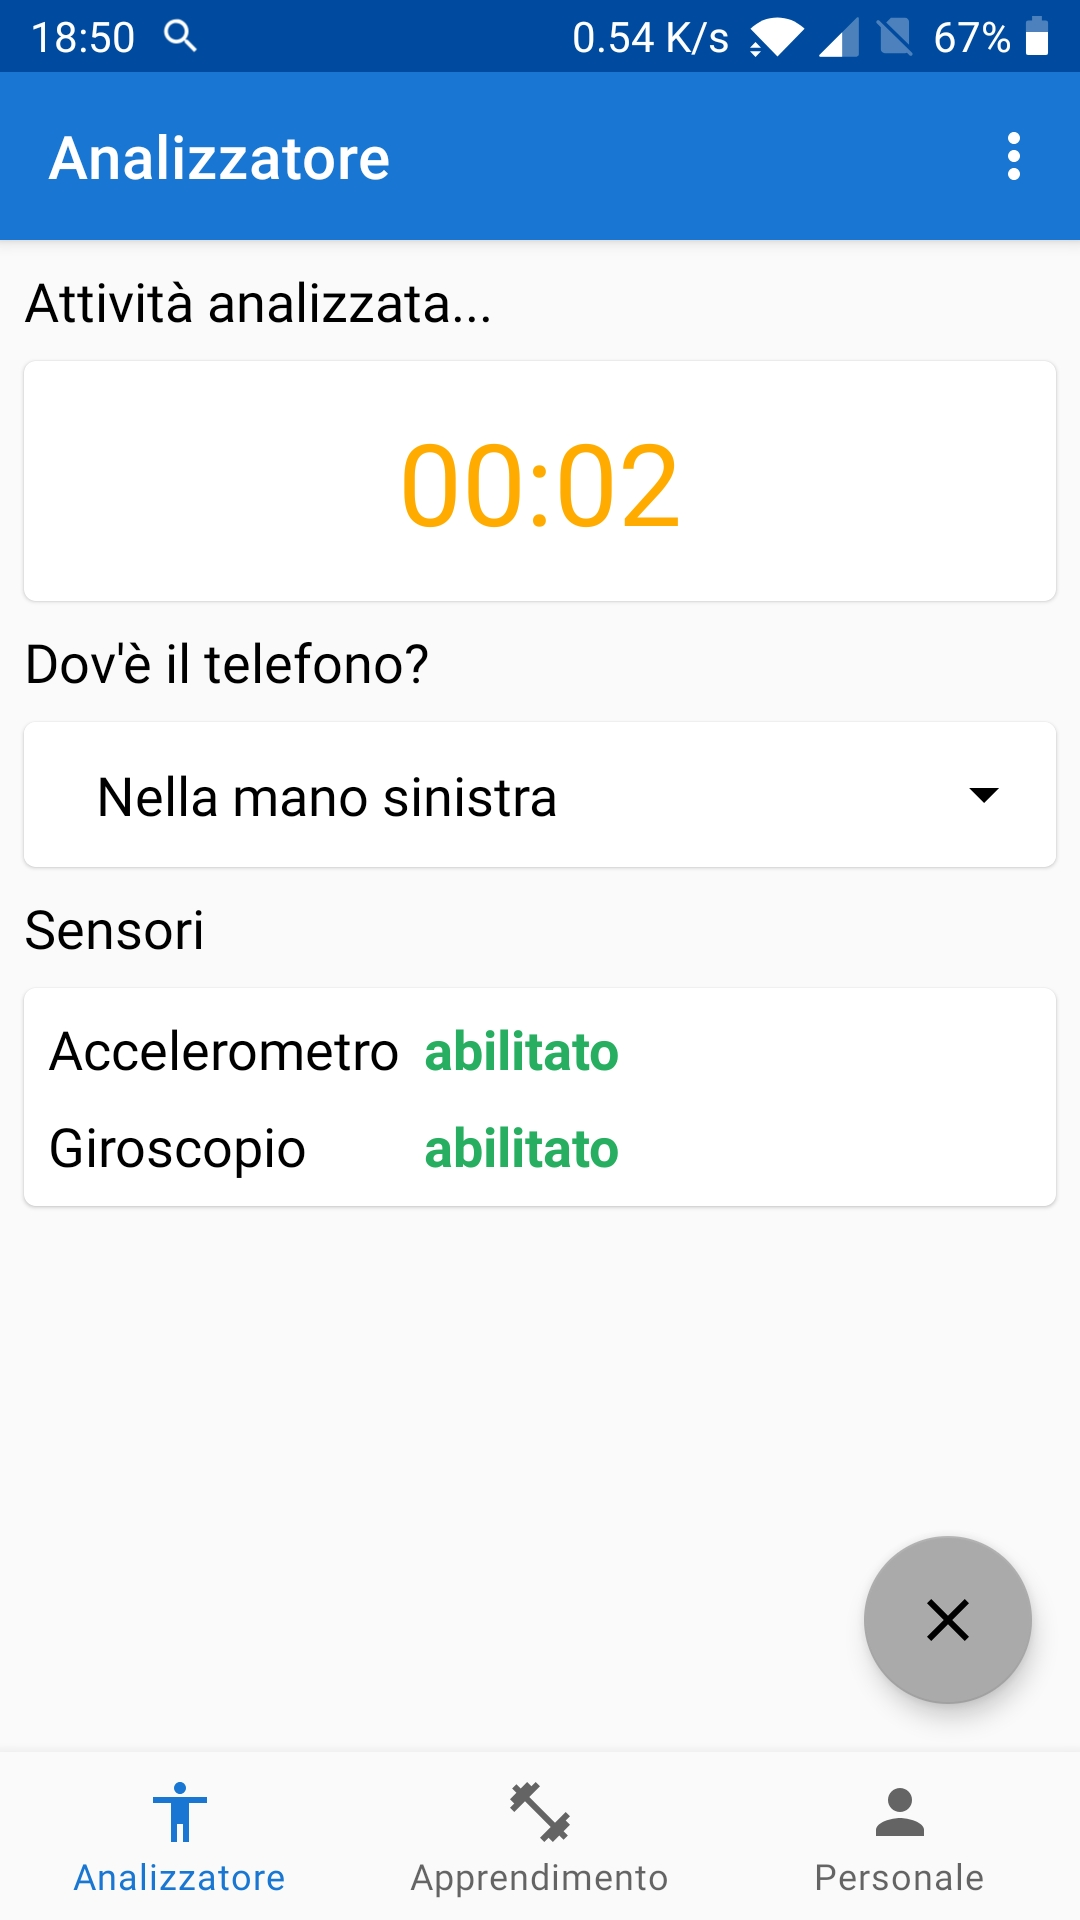
\includegraphics[scale = 0.1019]{assets/images/screenshots/1b_Preparation.jpg}
    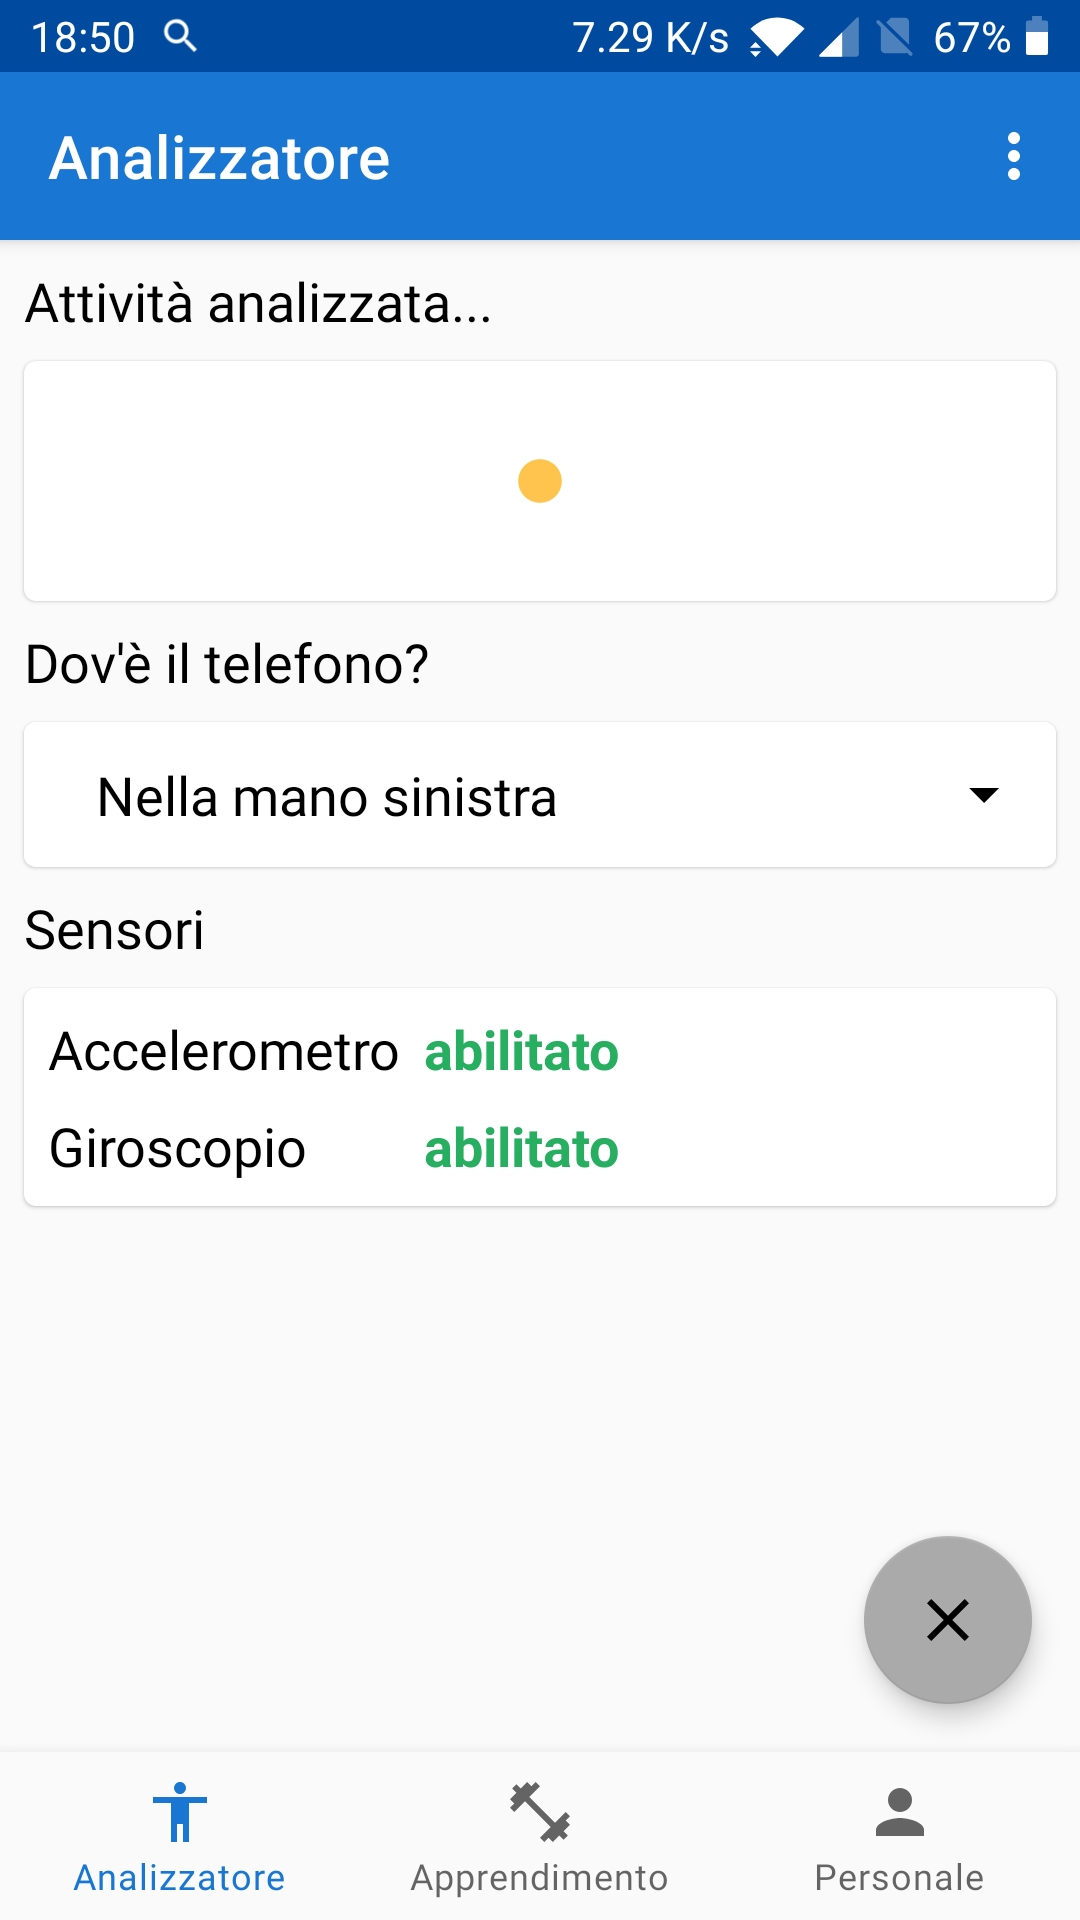
\includegraphics[scale = 0.1019]{assets/images/screenshots/1c_Analysis.jpg}
    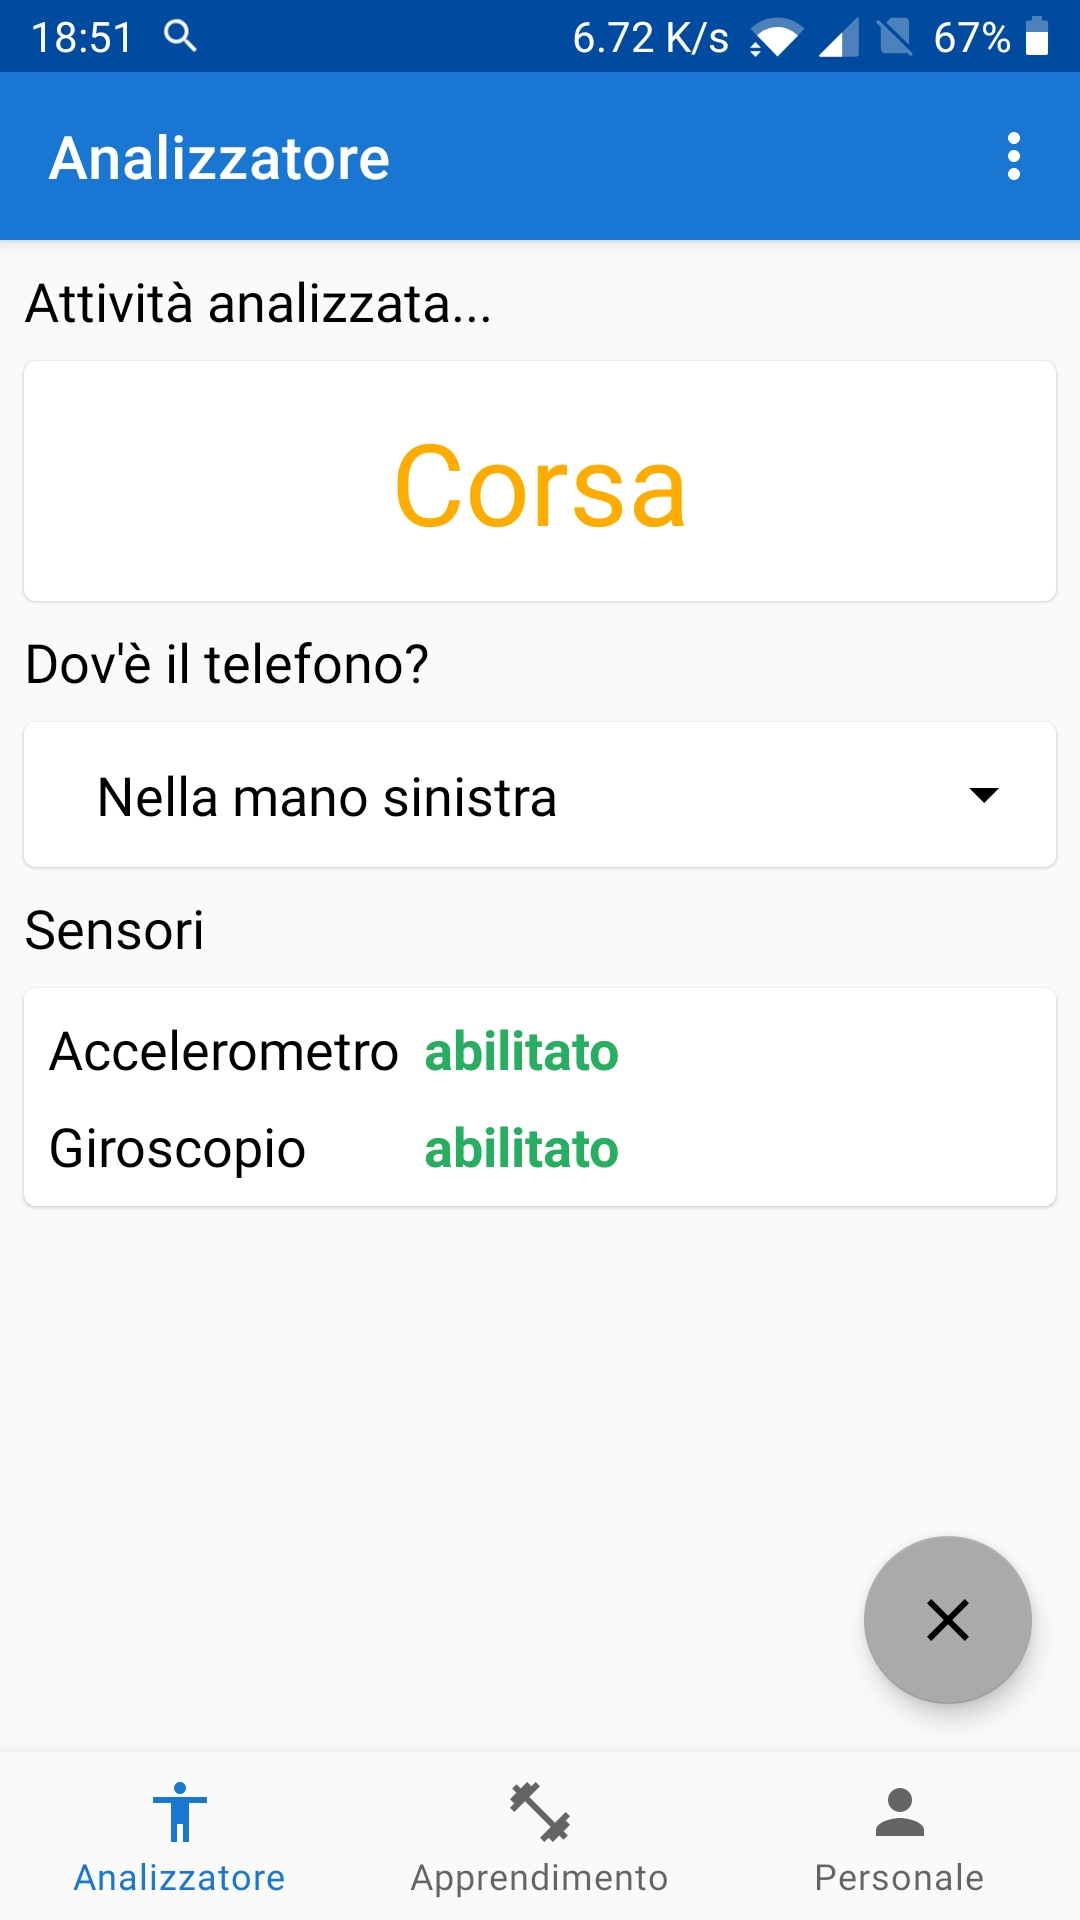
\includegraphics[scale = 0.1019]{assets/images/screenshots/1d_Prediction.jpg}
    \caption{Le 4 fasi dell'analisi}
    \label{fig:screenshots_analysis}
\end{figure}


\subsection{Sezione di apprendimento}
Nella sezione di apprendimento è possibile avviare un processo di raccolta dati del tutto simile a quanto appena visto, ma al quale si associa anche 
una attività tra quelle selezionabili.

L'obiettivo sarà poi quello di utilizzare questi dati sensoriali di cui si conosce la corrispondenza pratica per effettuare il \textit{train} 
della rete neurale da cui si genererà il modello. In questa fase si da piena fiducia all'utente sulla correttezza dei dati inseriti.

L'insieme delle azioni svolte in questa sezione sono divisibili in 3 fasi.

\subsubsection{Fase 1: Inizializzazione}
In questa prima fase l'applicazione scarica diverse informazioni tramite l'utilizzo delle API (viste nella sezione \ref{section:api}):
\begin{itemize}
    \item le informazioni relative alle posizioni del dispositivo selezionabili
    \item la lista di attività addestrabili e il tempo necessario per il loro apprendimento
\end{itemize}
Prima dell'avvio dell'apprendimento l'utilizzatore dovrà quindi selezionare sia la posizione in cui tenere il 
telefono durante l'esecuzione che l'attività da allenare.

\subsubsection{Fase 2: Preparazione}
Anche in questo frangente sarà inizializzato un servizio in foreground \cite{services} che si occuperà di svolgere 
tutte le azioni necessarie per le fasi seguenti e la UI continuerà ad essere aggiornata con le informazioni ricevute da questo servizio.

Nuovamente come prima cosa viene contattato il server per stabilire una connessione TCP ed una volta ricevuta risposta affermativa
sarà avviato il conto alla rovescia per la preparazione.

\subsubsection{Fase 3: Apprendimento}
Allo scadere del countdown sono avviati in parallelo un ulteriore conto alla rovescia e tutti i sensori per la raccolta dei dati.

Il secondo countdown indica il tempo di esecuzione necessario e potrebbe differire tra le diverse attività. Fino allo scadere del tempo tutti i dati 
raccolti dai sensori sono inviati al server.

\begin{figure}[H]
    \centering
    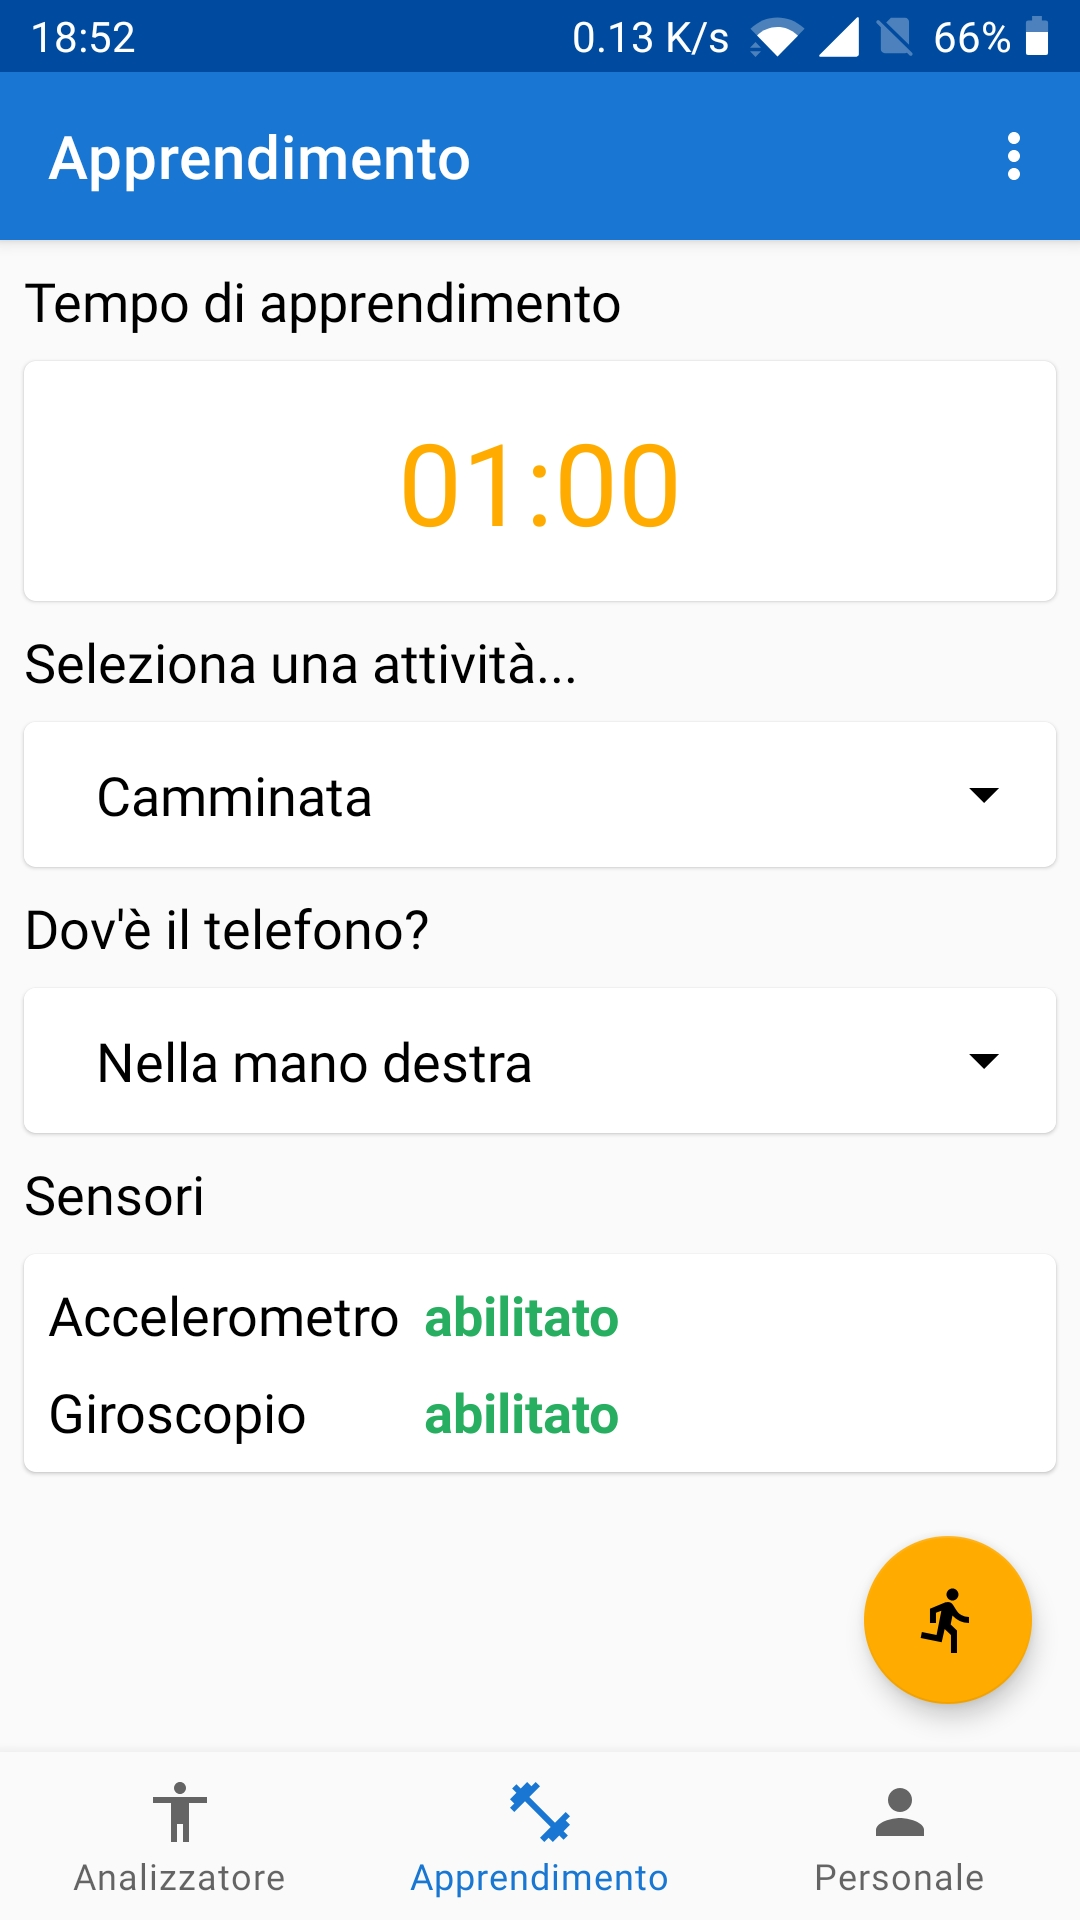
\includegraphics[scale = 0.1019]{assets/images/screenshots/2a_Init.jpg}
    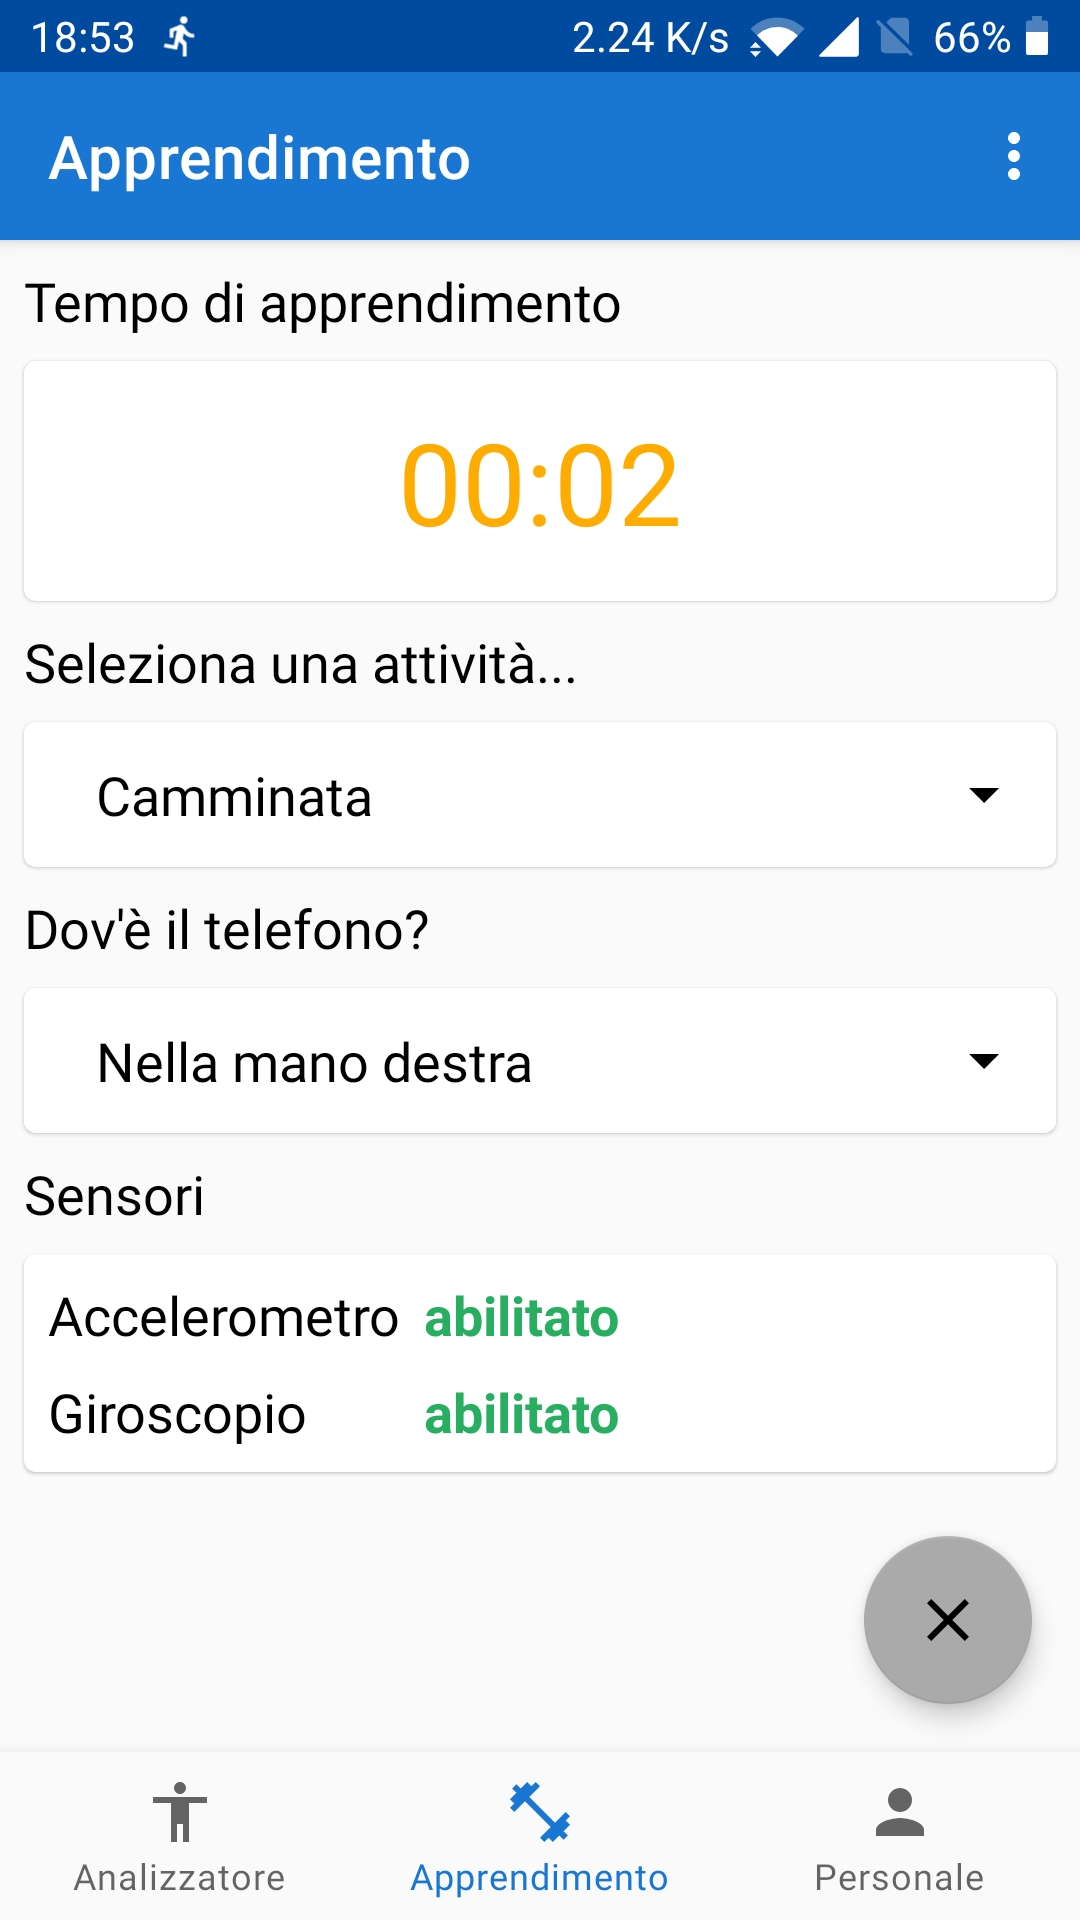
\includegraphics[scale = 0.1019]{assets/images/screenshots/2b_Preparation.jpg}
    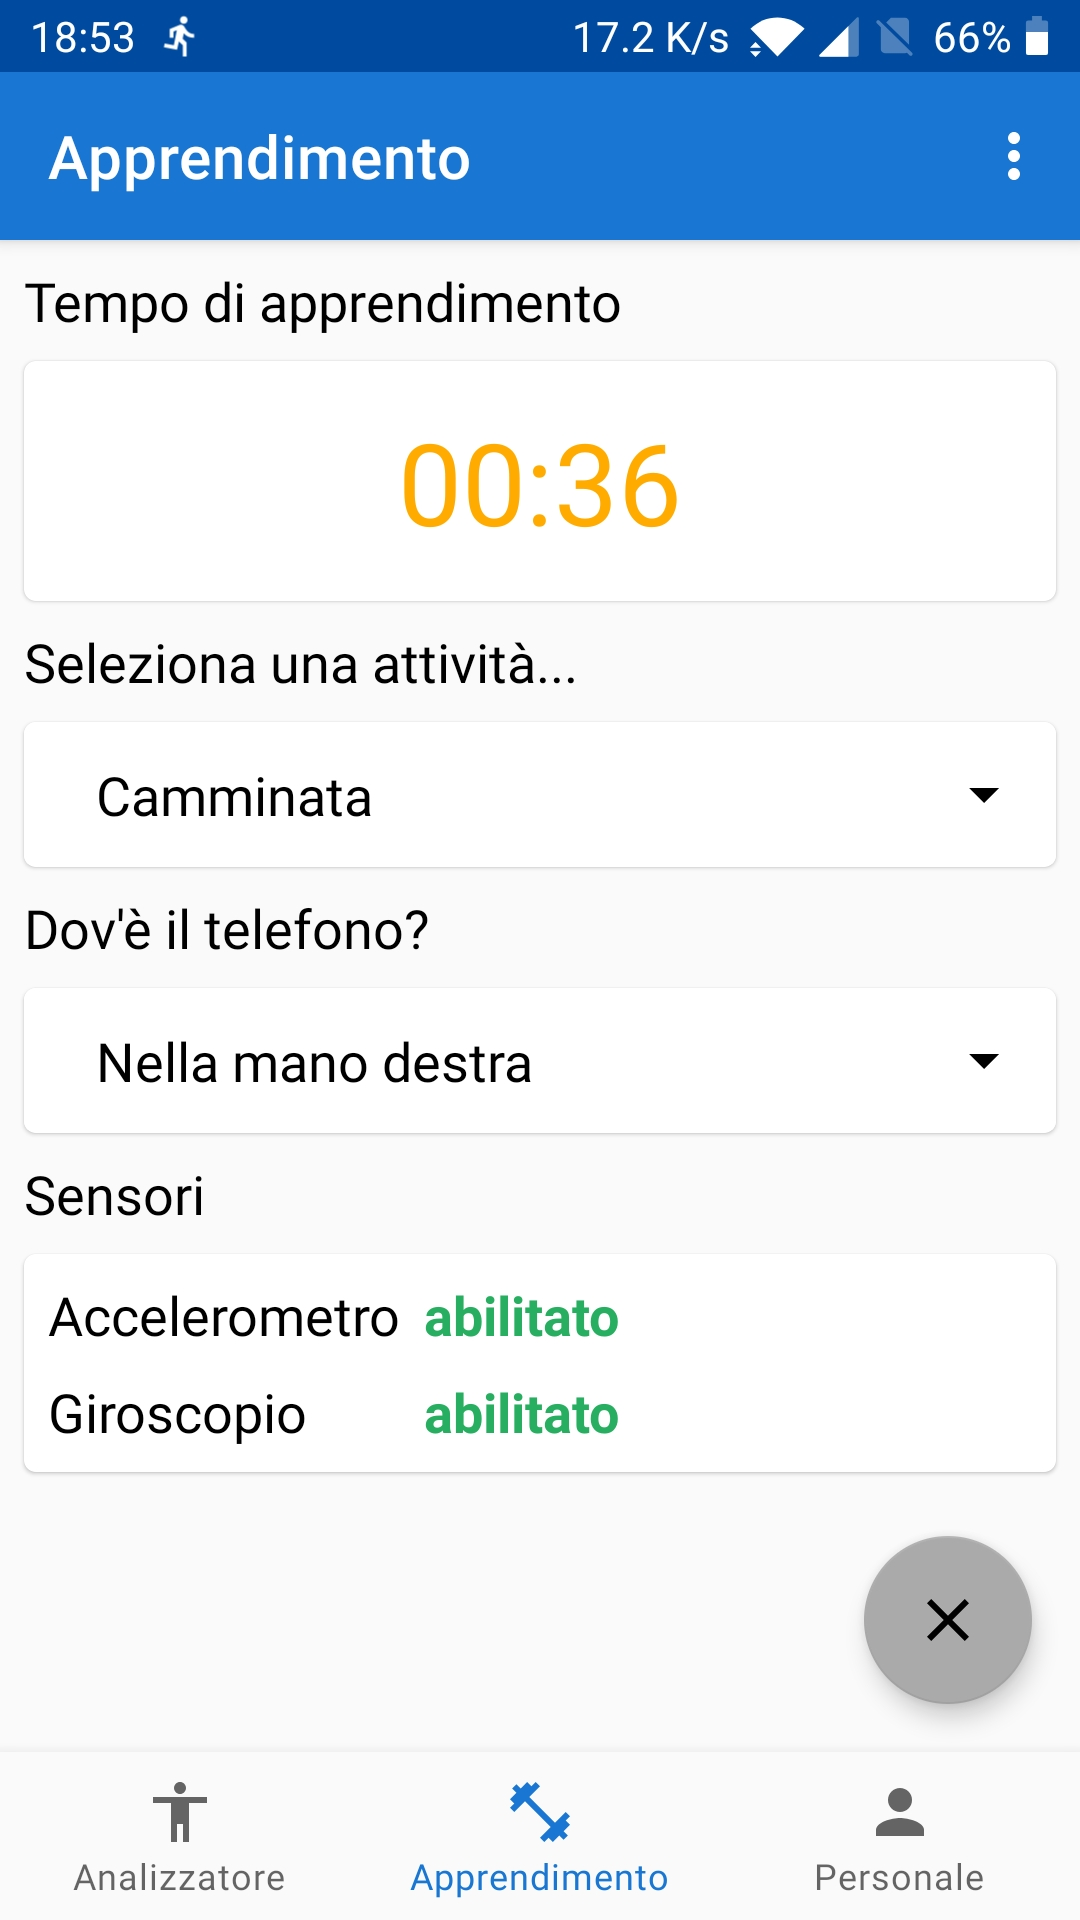
\includegraphics[scale = 0.1019]{assets/images/screenshots/2c_Learning.jpg}
    \caption{Le 3 fasi dell'apprendimento}
    \label{fig:screenshots_learning}
\end{figure}


\subsection{Sezione per l'inserimento di dati aggiuntivi}
La sezione è utile per dare la possibilità di inserire dati aggiuntivi che potrebbero essere utilizzati in qualche modo
dal classificatore. Un esempio possibile è la richiesta di dati fisici dell'utente (altezza, peso, etc.) qualora in futuro
si decidesse dar loro una rilevanza nella classificazione.

Malgrado agli occhi dell'utente appaia come un semplice modulo di inserimento dati, la sezione in questione è la più dinamica di tutti 
per quanto riguarda l'interfaccia. 
Il modulo che richiede all'utente i dati personali è generato programmativamente per intero a partire da quanto scaricato dal 
relativo endpoint delle API. Questa opportunità permette ad un amministratore di sistema di variare le richieste 
senza dover rilasciare un'aggiornamento dell'applicazione.

\begin{figure}[H]
    \centering
    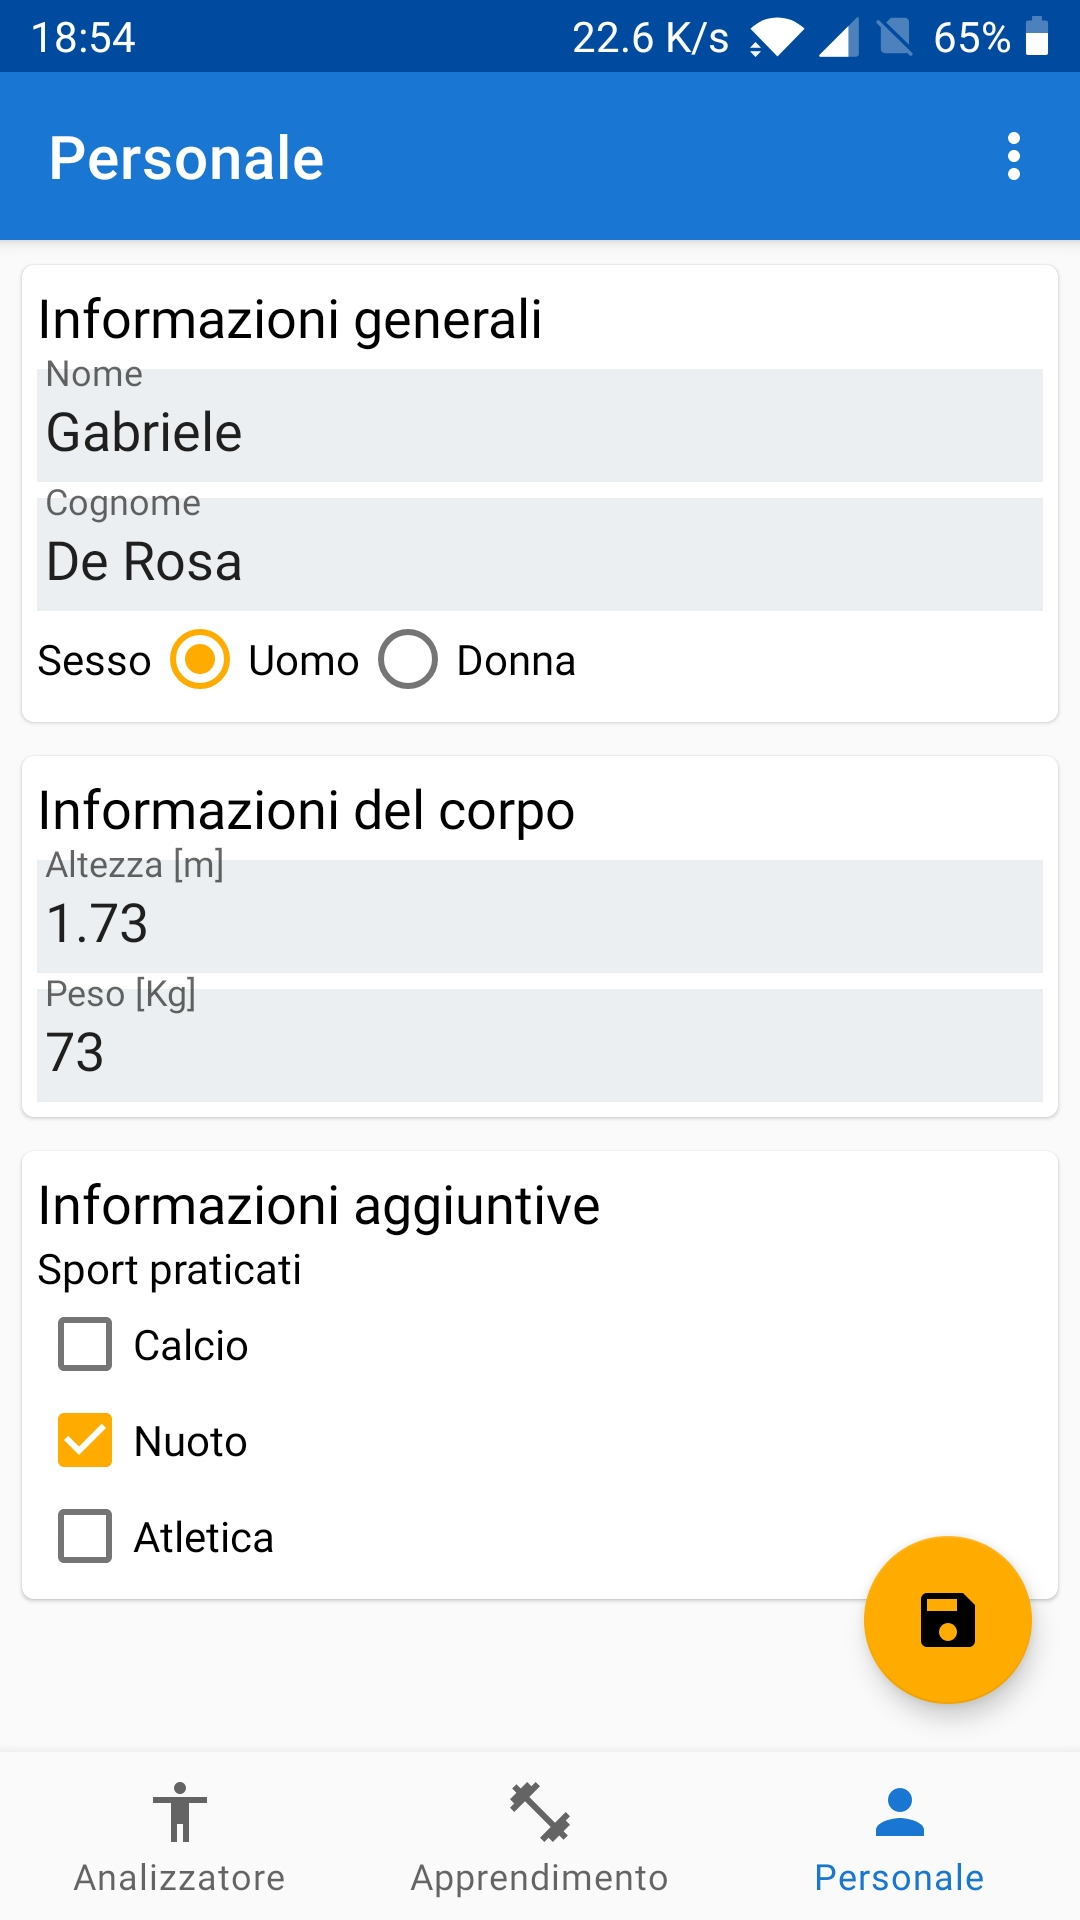
\includegraphics[scale = 0.1019]{assets/images/screenshots/3a_Init.jpg}    
    \caption{Il modulo di inserimento dati generato programmativamente}
    \label{fig:screenshots_personal}
\end{figure}



\section{Feedback sonoro}
Dal funzionamento che abbiamo appena visto è intuibile che l'app possa essere utilizzata con il dispositivo situato in posizioni che non permetterebbero
un collegamento visivo diretto. Quando la posizione selezionata è, per esempio, nelle tasche.

Tale situazione renderebbe impossibile l'accesso alle informazioni relative al progresso dell'attività in corso di esecuzione, che sia 
un'analisi o un apprendimento.
Questa eventualità ha reso necessaria l'implementazione di un feedback sonoro realizzato mediante le librerie 
di sintetizzazione vocale per il \textit{text to speech} \cite{tts} offerte da Android.

Oltre al feedback visivo è offerto quindi un feedback sonoro per tutte le informazioni rilevanti, come l'inizio e la fine dell'attività, 
il conto alla rovescia ed i risultati dell'attività ipotizzata.

\begin{listing}[H] 
    \inputminted[frame=single,framesep=10pt]{java}{snippets/app/voice.java}
    \caption{Implementazione del text to speech in Android}
\end{listing}



\section{Countdown Timers}
I countdown che regolano il tempo di svolgimento delle attività sono implementati utilizzando la 
classe \textit{CountDownTimer} \cite{countdown} offerta direttamente da Android.

I due timer implementati non hanno un tempo stabilito in partenza. I secondi utili per la preparazione possono essere facilmente
impostati dall'utente mediante un input nelle impostazioni. Il tempo per l'apprendimento dell'attività è invece scaricato dalle API
tramite le medesima richiesta delle informazioni sulle attività.

\begin{listing}[H] 
    \inputminted[frame=single,framesep=10pt]{java}{snippets/app/countdown.java}
    \caption{Implementazione di un conto alla rovescia}
\end{listing}



\section{Accesso alle API}
Le chiamate alle API, di cui abbiamo visto le varie applicazioni per l'ottenimento di dati informativi, 
sono fatte utilizzando la librerie Retrofit. Questa libreria, implementando le classi opportune associate ai dati
che ci si aspetta dalle risposte (\textit{API Response}), permette di ottenere facilmente le informazioni discusse.
\subsubsection{Retrofit}
Retrofit \cite{retrofit} è una librerie open source nata per trasformare una richiesta ad una REST API 
in una Java Interface.


\newpage
\section{Sensori di movimento}
I sensori di movimento implementati sono \textbf{accelerometro} e \textbf{giroscopio}.

Entrambi presentano gli stessi valori informativi (i tre assi x, y, z), pertanto durante lo sviluppo sono stati gestiti in modo analogo.

I sensori sono gestiti dal sistema operativo stesso. Per richiedere l'accesso è necessario fare richiesta al gestore (\textit{SensorManager}) 
per abilitare i sensori necessari ed implementare la classe \textit{SensorEventListener} \cite{sensor}
insieme ai \textit{callback} che saranno chiamati dal sistema ad ogni evento.
\subsubsection{Callback}
Una callback è una funzione richiamata dal sistema operativo quando si verifica un determinato evento, in modo da implementarne 
una gestione personalizzata.

\begin{listing}[H] 
    \inputminted[frame=single,framesep=10pt]{java}{snippets/app/sensors.java}
    \caption{Implementazione del callback dei sensori}
    \label{listing:sensor-event-callback}
\end{listing}



\newpage
\section{Comunicazioni con il server}
Oltre a ricavare le informazioni sensoriali è ovviamente necessario procedere al loro invio al server  
dove verranno processate come visto nella sezione \ref{section:receiver}.

Per prima cosa però è indispensabile avere una connessione attiva. Tale connessione è richiesta all'avvio dei servizi di 
analisi e apprendimento.

Come abbiamo precedentemente discusso si è scelta una connessione TCP via socket. La corrispondente implementazione Java
avviene proprio mediante la classe \textit{Socket} \cite{socket}.
\begin{listing}[H] 
    \inputminted[frame=single,framesep=10pt]{java}{snippets/app/server.java}
    \caption{Implementazione della connessione via socket}
\end{listing}
Una volta attiva la connessione è possibile procedere con l'invio dei dati ogni qual volta che il sistema 
operativo notifica un cambiamento di stato dei sensori mediante l'apposito callback 
di cui abbiamo visto l'implementazione.